
\section{Radial dam break on a dry bed}

A radial dam break test problem involving a dry bed. Should show a rarefaction fan. Note that the reference solution is found from the 1D FVM for SWE involving varying width and topography. See a paper of Roberts and Wilson~\cite{RW2011}.


\subsection{Results}

We should see excellent agreement between the reference and numerical solutions.

\begin{figure}
\begin{center}
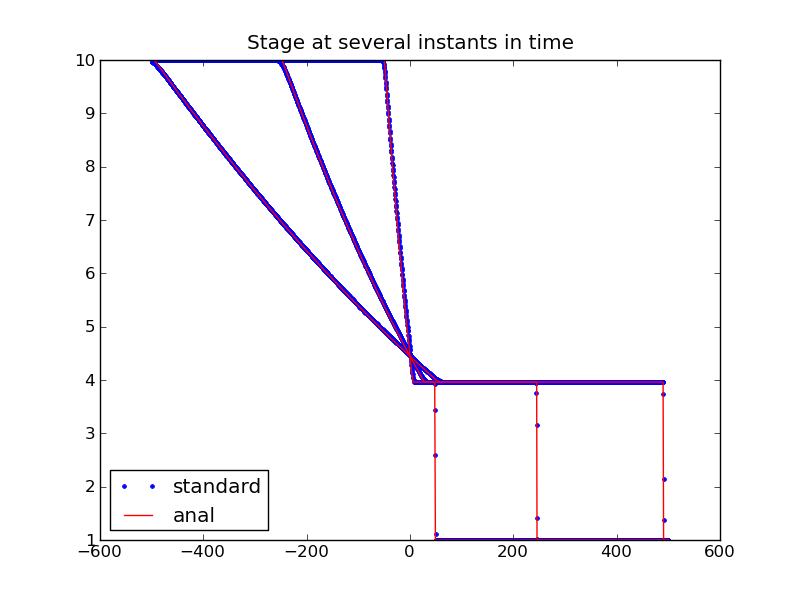
\includegraphics[width=0.9\textwidth]{stage_plot.png}
\end{center}
\caption{Stage results}
\end{figure}


\begin{figure}
\begin{center}
\includegraphics[width=0.9\textwidth]{rmom_plot.png}
\end{center}
\caption{Radial momentum results}
\end{figure}


\begin{figure}
\begin{center}
\includegraphics[width=0.9\textwidth]{rvel_plot.png}
\end{center}
\caption{Radial velocity results}
\end{figure}


\endinput
